\chapter{Алгоритм дифференциальной эволюции для задачи оптимизации фазированных антенных решеток}\label{sec:radio}

\section{Базовый вариант алгоритма}\label{sec:de:default}

Эволюционные алгоритмы~(ЭА) — один из наиболее широко используемых методов решения многоэкстремальных задач оптимизации,
применяемый во многих областях информатики, экономики, инженерии и др.
Дифференциальная эволюция~(ДЭ)~\cite{storn:de} — один из наиболее эффективных ЭА непрерывной оптимизации.
В частности, ДЭ была признана стратегией-победителем нескольких конкурсов по оптимизации~\cite{das:de}.
Подобно другим эволюционным алгоритмам, ДЭ вдохновлен естественным процессом эволюции и включает в себя применение мутаций,
рекомбинации и селекции. Основная особенность ДЭ заключается в том, что в этом алгоритме при построении особей-потомков
учитываются разницы между векторами,
присутствующими в популяции. В этом смысле он похож на алгоритм Нелдера-Мида~\cite{nelder:simplex} и метод CRS из~\cite{price:global}.

ДЭ -- рандомизированный алгоритм, основанный на популяционном поиске, в котором на каждой итерации вычисляется
новый набор пробных решений (векторов). В базовом варианте ДЭ для каждого члена
популяции~(их называют целевыми векторами) создается новый мутантный вектор.
Затем мутантный вектор комбинируют с целевым вектором для создания пробного вектора.
Наконец, применяется фаза селекции для выбора особей следующей популяции.
Таким образом, итерации ДЭ продолжаются, пока не будет достигнут критерий остановки.
В поколении $G$ $i$-й вектор популяции обозначается как $\textbf{X}_{i,G} = [x_{1,i,G}, x_{2,i,G}, ..., x_{D,i,G}]$.
Ниже приведены более подробные сведения о каждой фазе ДЭ.

Эксперименты показывают~\cite{storn:de_practical}, что в целом эволюция популяции такова, что
в случае попадания популяции в некоторый <<овраг>>, популяция ориентируется вдоль этого оврага и
математическое ожидание разности двух случайных векторов оказывается направленным вдоль оврага.
Это обеспечивает быстрое движение вдоль узких оврагов, тогда как для градиентных методов в
аналогичных условиях характерна колебательная динамика «от стенки к стенке». Приведенные эвристические
соображения иллюстрируют наиболее важную и привлекательную особенность алгоритма ДЭ -- способность динамически
адаптироваться к особенностям рельефа оптимизируемой функции. Именно этим объясняется способность алгоритма быстро проходить
сложные овраги, обеспечивающая его способность к поиску оптимальных или близких к оптиуму решений.

\paragraph*{Инициализация.}

ДЭ обычно начинает процесс оптимизации со случайно инициированной популяции, состоящей из $D$ векторов.
Поскольку информация о перспективности различных областей пространства решений, как правило, отсутствует,
для инициализации ДЭ применяются равномерные генераторы случайных векторов в параллелепипеде с некоторыми
границами $a_i$, $b_i$ по каждой координате
$j$, т.е. $j$-я компонента $i$-го вектора
инициализируется как $x_{j, i, 0} = a_{j} + rand_{i,j}(b_j - a_j )$,
где величина $rand_{i,j}$ выбрана с равномерным распределением между 0 и 1.

\paragraph*{Мутация.}

Для каждого целевого вектора создается мутантный вектор. В настоящее время известно несколько вариантов этого оператора.
В классическом варианте ДЭ применяется стратегия $rand/1$. В этом случае мутантный вектор $\textbf{V}_{i,G}$ создается следующим
образом:

\begin{equation}\label{eq:de_mut}
  \textbf{V}_{i,G} = \textbf{X}_{r_1,G} + F \cdot (\textbf{X}_{r_2,G} - \textbf{X}_{r_3,G}), \ r_1 \neq r_2 \neq r_3,
\end{equation}
где $r_1, r_2, r_3 $ -- попарно различные целые числа, случайно выбранные из множества $\{1,...,D\}\backslash i$.
Разница между векторами масштабируется множителем $F$, который
называется {\em силой мутации} и обычно определяется в интервале [0.4, 1].

\paragraph*{Рекомбинация.}

Для объединения информации о различных пробных решениях и с целью увеличения разнообразия в популяции применяется оператор
кроссинговера (рекомбинации). Каждый целевой вектор~$\textbf{X}_{i,G}$ рекомбинируется с соответствующим ему мутантным
вектором~$\textbf{V}_{i,G}$ для создания пробного решения $\textbf{U}_{i,G} = [u_{1,i,G}, u_{2,i,G}, ..., u_{D,i,G}]$.
Наиболее типичный вариант кроссинговера в ДЭ действует следующим образом:
\begin{equation}\label{eq:de_crossover}
  \textbf{u}_{j,i,G} =
    \begin{cases}
     v_{j,i,G}, & \mbox{если~} rand_{i,j} \leq CR \mbox{~или~} j = j_{rand} \\
     x_{j,i,G} & \mbox{иначе},
    \end{cases},
\end{equation}
где $rand_{i,j}$ -- равномерно на $[0, 1]$ распределенное случайное число, $j_{rand}$ -- случайно выбранный индекс. При этом
гарантируется, что $\textbf{U}_{i,G}$ наследует хотя бы одну компоненту от $\textbf{V}_{i,G}$. Параметр
$CR \in [0, 1]$ называется {\em интенсивностью кроссинговера}.

\paragraph*{Селекция.}

Наконец, выполняется отбор для определения следующего поколения. Каждый пробный вектор сравнивается с соответствующим
ему целевым вектором, и выживает лучший из них:

\begin{equation}\label{eq:de_sel}
  \textbf{X}_{i,G+1} =
  \begin{cases}
    \textbf{U}_{i,G}, & \mbox{если} \ \tilde{F}(\textbf{U}_{i,G}) \leq \tilde{F}(\textbf{X}_{i,G}) \\
    \textbf{X}_{i,G} & \mbox{иначе}.
  \end{cases}
\end{equation}

Таким образом, каждый член популяции либо становится лучше по целевой функции, либо остается с тем же значением
целевой функции в следующем поколении.

\section{Гибридный вариант алгоритма дифференциальной эволюции}
Будучи примененным к различным примерам из~\cite{tyu:daor}, описанный выше базовый вариант алгоритма
дифференциальной эволюции зачастую не мог обнаружить даже допустимых решений за все отведенное ему время.
Чтобы избежать этой тенденции, в данной работе предложен гибридный вариант ДЭ с использованием градиентного метода,
масштабированием решений в допустимую область и адаптацией штрафа, учитывающий специфику решаемой задачи.
К особи с лучшим значением целевой функции в гибридном алгоритме применяется градиентный алгоритм, когда 
%количество итераций алгоритма ДЭ превышает двухкратное количество его итераций, потребовавшееся для получения текущего рекорда или
исчерпано время счета, отведенное на ДЭ. 

%Комбинация ДЭ с градиентным подъемом реализуется следующей процедурой, выполняемой перед переходом к следующему поколению~$G+1$:
%
%\begin{flushleft}
%\small
%Пусть
%$G_0$ -- \verb"номер поколения, когда было последнее улучшение рекорда,"\\
%$Grad(X)$ -- \verb"результат применения градиентного подъема с начальным решением "$X,$\\
%$X_G$ -- \verb"лучшая особь популяции на итерации "$G.$\\
%$\mbox{ }$\\
%
%\textit{Если} $G > D$ \textit{и} $G > 2 G_0,$ \textit{то положить} \\
%\leftskip=12pt
%    $X' := Grad(X_G).$\\
%    \textit{Если} $X'$ = $X_G,$ \textit{то} \verb"завершить выполнение алгоритма, выдать решение" $X_G.$\\
%    \textit{Иначе положить} \\
%    \leftskip=24pt
%        $X_G := X',$\\
%        $G_0 := G.$\\
%        \leftskip=12pt
%\end{flushleft}
%Условие $G > 2 G_0$ показывает отсутствие улучшения рекордного значения целевой функции за то же число итераций,
%которое было затрачено на получение этого рекорда.
%Условие $G > D$ гарантирует, что на начальных итерациях ДЭ не будет принято решение о запуске градиентного
%алгоритма~\cite{BN98,HK93}. Здесь и далее под улучшением рекордного значения понимается увеличение лучшего
%найденного значения целевой функции в очередном поколении~$G$ не менее, чем на~$\varepsilon$, где параметр $\varepsilon$
%тот же, что и в критерии остановки градиентного алгоритма (по минимальному допустимому приращению целевой функции)~\cite{tyu:daor}.

\paragraph*{Масштабирование решений.}
Для рассматриваемой задачи существует преобразование, позволяющее привести к
допустимой области любое решение $\textbf{x}$, которое нарушает только неравенства задачи~(\ref{eq:task3}) вида
$\textbf{x}^{T}\textbf{H}^{(k)}\textbf{x} \leq 1$:

\begin{equation}
    \textbf{x}': =\alpha(\textbf{x})^{-1/2} \textbf{x} ,
    \label{eq:scale}
\end{equation}
где $\alpha(\textbf{x}):=\max_{k=\overline{1,n}} \textbf{x}^T \textbf{H}^{(k)}\textbf{x}$. Поскольку как целевая функция, так и
ограничения представлены квадратичными формами, применение такой операции приведет к пропорциональному уменьшению
в~$\alpha(\textbf{x})$ раз значений каждой из квадратичных форм. Другими словами, если в некоторой точке $\textbf{x}$
значения каждой из квадратичных форм, задающих ограничения, больше 0, причем значения некоторых из них
больше 1, то по формуле (\ref{eq:scale}) можно определить множитель, умножение которого на вектор $\textbf{x}$ ведет к тому,
что наибольшее из значений квадратичных форм, задающих ограничения, будет равно 1. Данная процедура применяется для
выбора начального решения, а также для масштабирования каждого нового решения перед оценкой его качества в алгоритме ДЭ
и после завершения градиентного подъема.
При этом, если решение до масштабирования имело большие нарушения ограничений, то после масштабирования его целевая функция
существенно изменяется (как правило, в сторону снижения качества).
На этом принципе основано адаптивное правило подбора штрафного коэффициента~$r$, описываемое далее.

% Кроме того, для улучшения качества решений в гибридном варианте предлагается динамическое увеличение штрафного коэффициента:

\begin{flushleft}
\small
Пусть
$G$ -- \verb"номер текущей итерации," \\
$G_0$ -- \verb"номер итерации, на которой было получено улучшение рекорда,"\\
$G_1$ -- \verb"номер итерации, на которой произошло предыдущее увеличение штрафа,"\\
%$D$ -- \verb"размер популяции,"\\
$r$ -- \verb"текущее значение штрафного коэффициента."\\
$\mbox{ }$\\

\textit{Если} $G > D$ \textit{и} $G > 1.5 G_0$ \textit{и} $G > 2 G_1,$  \textit{то положить} \\
\leftskip=12pt
    $r := 2r$\\
    $G_1 := G.$\\
    \leftskip=0pt
\end{flushleft}

Таким образом, при отсутствии существенных улучшений качества решений на протяжении $G_0/2$ итераций, еще до
вызова градиентного алгоритма и до окончания работы ДЭ делается попытка улучшить найденный результат за счет увеличения штрафа.
Условие $G > D$ гарантирует, что на начальных итерациях не будет принято решение об увеличении штрафа.
%, а условие $G > 1.5 G_0$ означает что рекордное значение целевой функции не было улучшено за $G_0/2$ итераций.
Условие $G > 2 G_1$ вводится для того, чтобы штрафной коэффициент не увеличивался слишком часто.
%Таким образом, при отсутствии существенных улучшений качества решений происходит увеличение штрафного коэффициента.
С учетом масштабирования особей в допустимую область, описанный механизм увеличения штрафа, как правило,
приводит к выживанию особей с меньшим нарушением ограничений и позволяет улучшить качество получаемых решений.
Как отмечено далее в~п.~\ref{sec:exp:de}, предложенная процедура адаптации штрафа приводит к сокращению погрешности получаемых решений.

\section{Вычислительный эксперимент}\label{sec:exp:de}

Вычислительный эксперимент был поставлен для задач, рассмотренных в~\cite{tyu:daor,tyu22:ring}. В данной
статье ШВИК, ШВДК, СВДК обозначают решетки кольцевой структуры. Далее следует указание количества элементов (8 или 16).
Через тире -- расстояние (метры) от центра излучателя до центра решетки (15, 20, 25, 30, 37). Для ШВД приводится плотность противовесов (например, 3:3). Поскольку современные ЭВМ на аппаратном уровне поддерживают вычисление в параллельном режиме, рассматриваемый здесь алгоритм ДЭ был адаптирован под эту особенность: за один запуск алгоритма производится 4 параллельных выполнения, а на выход подается лучшее решение. Это позволяет использовать возможности современных ЭВМ для получения более качественных решений.
В таблице~\ref{tab:results_de} результаты, полученные с помощью градиентного подъема из~\cite{tyu:daor} и гибридного алгоритма дифференциальной эволюции~(ДЭ),
сравниваются с результатами коммерческого решателя BARON версии~18.11.12 из пакета GAMS.
%В колонке BARON* показаны результаты, полученные решателем BARON при учете фазовой симметрии. Для ДЭ также были произведены эксперименты при учете симметрии, однако, их результаты практически идентичны результатам ДЭ без учета симметрии, поэтому, в таблице~\ref{tab:results_de} они не приводятся. Поскольку решатель BARON в пакете GAMS в режиме по умолчанию имеет ограничение по времени 1000с., ДЭ также использует этот лимит.
Все сравниваемые алгоритмы имеют ограничение по времени счета 1000с (эта длительность выбрана из практических соображений, т.к. она сопоставима с временем построения исходных данных с использованием системы NEC, и совпадает с ограничением по времени, выбранным в~\cite{tyu:daor}).
%В случае, если ДЭ получит решение раньше установленного временн\'{о}го ограничения, производится повторный запуск алгоритма до тех пор, пока это ограничение не будет исчерпано. За
В случае нескольких запусков ДЭ за отведенное время, за окончательное решение принимается лучшее из найденных за 1000с.
Для оценки среднего значения целевой функции на выходе ДЭ производилась серия из 10 независимых испытаний по
1000с в каждом. Эксперимент с гибридным алгоритмом ДЭ проводился при выборе типичных значений настраиваемых параметров
(популяция из 100 особей, $F=0.6$, $CR=0.6$). Значения целевой функции в таблице округлены до целых.
Полужирным шрифтом выделены случаи, когда указанное значение целевой функции не менее, чем на 1\% выше, чем у других алгоритмов.
Вычисления производились на ЭВМ с процессором Intel i7 (тактовая частота: 2.8ГГц), ОЗУ: 16Гб. 


\begin{table}[!h]

\centering
\caption{ Результаты градиентного подъема, гибридного алгоритма ДЭ и BARON}
\begin{tabular}{|c|c|c|cc|c c|}
    \hline
    \multirow{2}{*}{\textbf{Тип}} & \textbf{град. подъем} & \textbf{ДЭ} & \multicolumn{2}{|c|}{\textbf{BARON}} \\
    & \textbf{$\tilde{F}$} & \textbf{$\tilde{F}$} & \textbf{$\tilde{F}$} & \textbf{t, c}  \\
    \hline
    ШВИ 2х2         & ${138}$  & ${139}$   & 139    & 0.12      \\
    ШВИ 3х3         & ${576}$ & ${580}$   & 580    & 0.34       \\
    ШВД 2х2         & ${460}$ & ${463}$   & 463    & 0.27     \\
    ШВД 3х3         & ${915}$ & ${924}$   & 925    & 0.34        \\
    СВД 2х2        & ${357}$  & ${361}$   & 361    & 0.16         \\
    СВД 3х3        & ${1138}$ & 1163  & $\mathbf{1261}$   & 0.38     \\
    СВД 5х5        & ${5318}$  & $\mathbf{7132}$  & 6716   & 1000   \\
    СВД' 2х2       & ${233}$ & 198   & $\mathbf{253}$    & 0.25         \\
    СВД' 3х3       & ${664}$ & 834   & $\mathbf{1153}$   & 1.4          \\
    СВД' 5х5       & ${1382}$  & $\mathbf{2755}$  & 33     & 217.94     \\
    ШВИК 8-15(3:3) & ${217}$  & ${218}$   & 218    & 0.23       \\
    ШВИК 16-15(3:7)& ${727}$  & ${732}$   & 734    & 1.37     \\
    ШВИК 8-15(2:3) & ${1536}$  & $\mathbf{1664}$     & -   & 14.62     \\
    ШВДК 8-20      & ${1454}$  & ${1454}$  & 1455   & 2.78       \\
    ШВДК 8-30      & ${2422}$  & ${2422}$  & 2422   & 1.47     \\
    СВДК 8-25      & ${740}$  & ${740}$   & 740    & 0.23        \\
    СВДК 8-37      & ${1487}$  & ${1487}$  & 1487   & 0.23      \\
    \hline
\end{tabular}
\label{tab:results_de}
\end{table}

При увеличении числа испытаний до~20, на всех задачах, кроме СВД~3х3,  СВД'~2х2, СВД' 3х3 и ШВИК 16-15(3:7), гибридный алгоритм в 100\% испытаний находил решение, не отличающееся от лушего известного  более чем на 1\% по целевой функции. На примере ШВИК 16-15(3:7) частота получения указанного в таблице решения составлила~0.95. 
В соответствии с подходом из~\cite{GK},
на каждой задаче тестирование гибридного алгоритма может рассматриваться
как последовательность из 20 испытаний по схеме Бернулли, где
успехом считается получение решения, отличающееся от лучшего известного решения не более чем на 1\% по целевой функции.
Для указанной схемы Бернулли известны
оценки доверительного интервала вероятности
успеха $p^*$, которые являются асимптотически точными,
когда число испытаний стремится к бесконечности~\cite{Kramer}.
При конечном числе испытаний с использованием утверждения~1 из~\cite{eremeev:confidence} для случая биномиального распределения 
 может быть найден односторонний доверительный интервал для вероятности успеха $p^*$: при доверительном уровне 95\%
вероятность нахождения лучшего известного решения для любой из рассмотренных задач, кроме СВД~3х3,  СВД'~2х2, СВД' 3х3 и ШВИК 16-15(3:7), 
составляет не менее 0.861, а для задачи ШВИК 16-15(3:7) эта вероятность составляет не менее 0.784. Для оставшихся трех задач содержательной нижней оценки для $p^*$ не получено. 

%Также в результате проведенных экспериментов были получены другие результаты, не отраженные в таблице~\ref{tab:results_de} для краткости изложения.
Aналогичные испытания производились и с помощью решателя ANTIGONE версии~39.1.0 в пакете GAMS, однако, было выявлено, что в режиме по умолчанию данный решатель на всех задачах выдал нулевое решение, кроме СВД~2х2, где решение по целевой функции совпадало с результатом BARON. Как правило, время, потребовавшееся для нахождения рекордного значения с помощью ДЭ отличалось незначительно от выбранного веременн\'{о}го ограничения.

Также, в результате проведенных экспериментов было обнаружено, что динамическая адаптация штрафного коэффициента позволяет ДЭ достичь более качественных решений.
%, что особенно заметно в тех случаях, когда результаты ДЭ и BARON близки по качеству. 
В частности, сравнение результатов гибридного ДЭ при адаптации штрафа с результатами предварительных экспериментов с гибридным ДЭ, проведенных до реализации процедуры адаптации штрафа (при прочих равных условиях), показывают, что на всех примерах, кроме СВД'3x3, результаты предварительных экспериментов уступали по качеству решений.  

С целью изучения возможности ускорения работы решателей за счет учета специфики задачи были проведены дополнительные исследования
структуры рассматриваемых примеров с точки зрения линейных симметрий этих задач~\cite{yurkov:symmetry}.
Ранее было отмечено (см.~\cite{tyu:daor}), что решения рассматриваемой задачи эквивалентны с точностью до сдвига
фаз во всех излучателях на равную величину.
Учет данной симметрии (для краткости называемой <<фазовой симметрией>>) может
быть реализован фиксацией в ноль одной из переменных задачи, например, $x_1=0$.
В результате добавления такого ограничения к условиям задачи число переменных сокращается
на единицу и можно предположить, что это сократит время вычислений для известных алгоритмов.
Нами поставлены вопросы о том, действительно ли происходит сокращение времени вычислений и о
существовании других семейств симметрий, которые могли бы еще более сократить пространство поиска решаемой задачи.

Для ответа на первый вопрос на всех тестовых примерах был найден коэффициент ускорения решателя BARON,
получаемый от фиксации $x_1=0$. Результаты представлены на рисунке~1 (здесь отсутствует задача СВД' 5х5, где
алгоритм с фиксацией затратил существенно большее время, но при этом нашел решение с большим на 10\% значением
целевой функции, а также задача ШВИК 8-15(2:3), в которой решения не были найдены в обоих случаях).
 большинстве примеров фиксация переменной привела к ускорению работы алгоритма, среднее ускорение по
представленным здесь задачам составило 0.95, что говорит о целесообразности фиксации в ноль одной из переменных
при использовании решателя. Аналогичный эксперимент с алгоритмом ДЭ и решателем ANTIGONE не показал существенного
улучшения качества решений или их ускорения в результате фиксации~$x_1$.

Для ответа на второй вопрос был проведен поиск непрерывой группы линейных симметрий в рассматриваемых примерах,
как описано в~\cite{yurkov:symmetry}. В результате было установлено, что других непрерывных семейств линейных
симметрий в рассматриваемых примерах не существует. Вопрос о поиске дискретных симметрий остается открытым.

\begin{figure}
\center{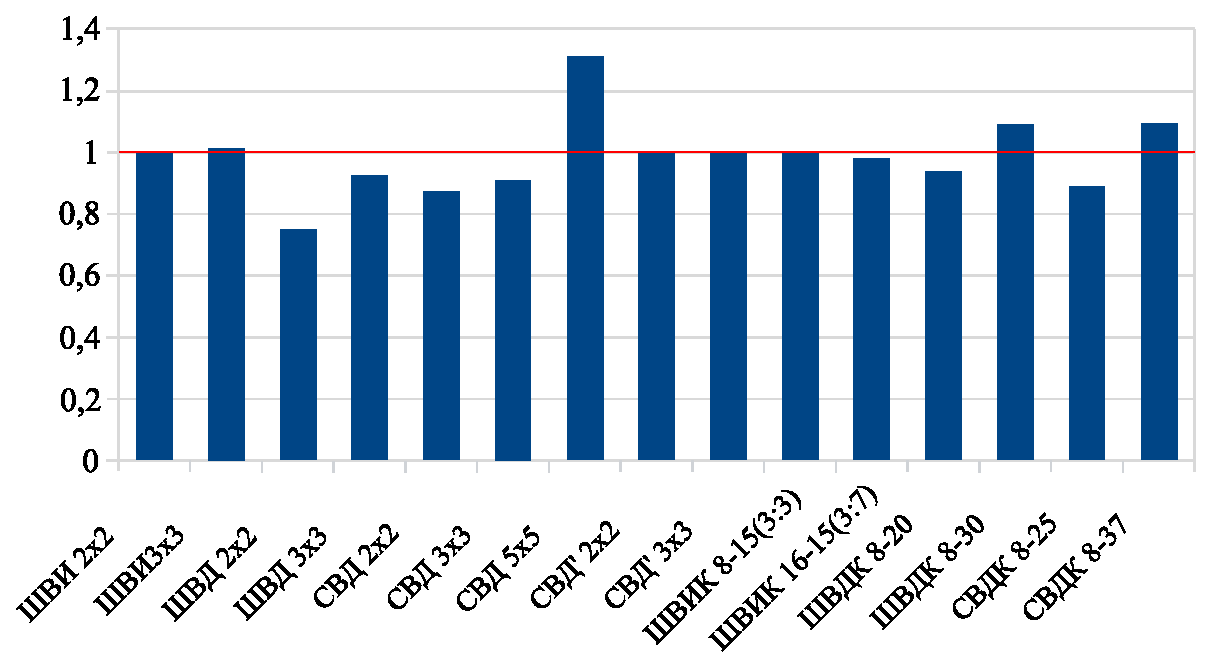
\includegraphics[width=0.95\linewidth]{ratio.eps}}
\caption{Отношение длительности вычислений с фиксацией первой координаты к исходной длительности вычислений}
\label{ris:ring}
\end{figure}

Из проведенных экспериментов можно сделать следующие выводы:\\
%\begin{itemize}
%  \item
1) разработанный в рамках данной работы гибридный вариант ДЭ показывает конкурентоспособные результаты по сравнению с коммерческим решателем BARON в режиме его настроек по умолчанию, при этом преимущество ДЭ наблюдается на задачах с наибольшей размерностью (50 и 16 переменных);\\
2) решатель ANTIGONE в режиме его настроек по умолчанию в большинстве тестовых примеров давал нулевое решение;\\
3) учет фазовых симметрий задачи~(\ref{eq:task1}) в большинстве случаев позволяет ускорить работу решателя BARON.\\
%4) других непрерывных семейств линейных симметрий в рассматриваемых задачах не существует.
%\end{itemize}

\section{Заключение}\label{sec:conclusion}

В рамках данной работы был разработан гибридный вариант алгоритма дифференциальной эволюции с использованием
градиентного алгоритма и адаптацией штрафа. Показано, что разработанный вариант ДЭ демонстрирует конкурентоспособные результаты, в
особенности на задачах большой размерности. Произведено сравнение гибридного алгоритма и коммерческих решателей с
учетом фазовой симметрии, имеющейся в рассматриваемой задаче, и без нее. В ходе эксперимента, учет симметрии в большинстве
случаев приводил к ускорению работы решателя BARON.

Результаты данного раздела были представлены в~\cite{tyu:msim22,tyu:reis}.
